\documentclass{article}
\usepackage[margin=1in]{geometry} 
\usepackage{amsmath,amsthm,amssymb,amsfonts, fancyhdr, color, comment, graphicx, environ}
\usepackage{xcolor}
\usepackage{mdframed}
\usepackage[shortlabels]{enumitem}
\usepackage{indentfirst}
\usepackage{hyperref}
\usepackage{graphicx}
\usepackage{float}
\usepackage{upquote}

\hypersetup{
    colorlinks=true,
    linkcolor=blue,
    filecolor=magenta,      
    urlcolor=blue,
}


\pagestyle{fancy}

\newcounter{question}
\newenvironment{question}
    { \begin{mdframed}[backgroundcolor=gray!20] \textbf{Question \arabic{question} : } \stepcounter{question} \\}
    {  \end{mdframed}}

\newenvironment{warning}
    { \begin{mdframed}[backgroundcolor=blue!20] \textbf{Warning : } }
    {  \end{mdframed}}
    
\newenvironment{info}
    { \begin{mdframed}[backgroundcolor=brown!20] \itshape }
    {  \end{mdframed}}

\newenvironment{code}
    { \begin{mdframed} }    {  \end{mdframed}}



\renewcommand{\qed}{\quad\qedsymbol}

% prevent line break in inline mode
\binoppenalty=\maxdimen
\relpenalty=\maxdimen

%%%%%%%%%%%%%%%%%%%%%%%%%%%%%%%%%%%%%%%%%%%%%
%Fill in the appropriate information below
\rhead{ISEP - II 3502} 
\chead{\textbf{Lab : Introduction to Apache Kafka}}
%%%%%%%%%%%%%%%%%%%%%%%%%%%%%%%%%%%%%%%%%%%%%

\begin{document}
\title{II 3502 - Lab : Introduction to Apache Kafka}
\author{Hervé RIVIERE - rivere.herve.isep@gmail.com}
\date{January 2022}
\maketitle


\section{Lab report : grade, format and due date}

You need to provide a lab report containing answer of the lab question before \underline{Friday January 21th, 23:59}.

\vspace{5mm}
This lab report : 
\begin{enumerate}
\item Should be uploaded in Moodle / II 3502 course / Kafka lab report box
\item Should follows the template (md file) \url{https://raw.githubusercontent.com/HerveRiviere/isep-kafka-lab/master/lab_report_template.md}
\item Will be grade with letter notation : A+ : fully completed with good answers and bonus part / A Fully completed without the bonus part / B - C : Partially completed or some incorrect answers / D : not received.
\item Will provide you \underline{up to 1 point to the final module grade}
\end{enumerate}
\vspace{5mm}
Don't hesitate to reach the teacher for any help or question about this lab. 
\begin{enumerate}
    \item by Microsoft Teams chat  : during the lab and up to report due date
    \item by email (rivere.herve.isep@gmail.com)
\end{enumerate}

\vspace{5mm}

Answers of all questions will be posted on Moodle one week after the lab.

\section{Kafka use cases}
\begin{question}
  Indicate if Apache Kafka can fit \underline{or not} with the following use cases : 
\begin{enumerate}
\item Server log aggregation (being able to collect and read log or events from multiple servers and / or applications)
\item Transfert of files (from couple of kB to GB) between servers and / or applications 
\item Event bus allowing distinct applications to share and consume events (example : a web server is producing login events and we want the anti-fraud application and the CRM can react to this events) 
\item Event store allowing to store (and if needed, reread in the same order) events produced by an application
\item Database (like MySQL or PostgresSQL)
\item Messaging system (like What's app or Hangout)
\item Make data pipeline / streaming ETL (for instance transfert specific records from a database to Elastic Search and to a file in a FTP)
\end{enumerate}
 
\end{question}
\begin{question}
What's a Kafka topic ? 
\end{question}

\begin{question}
True or false ? \\
An event inside Kafka can be modified ?
\end{question}

\section{The lab environement : a fully configured remote desktop}
A server with Apache Guacamole (web browser remote desktop solution) was configured for each student. Therefore only a web browser like Chrome or Firefox is needed.


If not yet given, ask the instructor for ip, username and password. 

\begin{warning}
Be careful with keyboard shortcuts and copy and paste commands : copy and paste will only work inside the remote desktop.\\
\textbf{For Mac users} : Please use "Windows like" shortcuts inside the remote desktop (so CTRL + C and not CMD +C)  
\end{warning}

\begin{warning}
For copy-past inside the remote desktop, best is to open this PDF in Chromium inside the remote desktop (file on the desktop)
\end{warning}

\begin{warning}
For pasting shell command inside a terminal you can use the following shortcut CTRL + SHIFT + V.
\end{warning}

\subsection{The lab environment}

The lab environment is simulating a multi-servers kafka infrastucture. It contains 
\begin{itemize}
\item A running zookeeper server (port 2181)
\item Three running kafka servers - a kafka server is often called also a kafka broker  (port 9092, 9093 and 9094)
\item Basic monitoring of the Kafka servers using prometheus (port 9090) 
\item A java IDE (InteliJ) with some java classes to interact with the Kafka cluster
\end{itemize}

Machine is connected to internet and your user has paswordless root permission

\begin{warning}
Having only one Zookeeper and multiple kafka brokers in a same server is a setup only valid for dev / experimental use cases. In a production grade environment each of these components will be on separate hosts and Zookeeper will be at least deployed on three servers.
\end{warning}

\subsection{Source code}
All the java code used in this lab and also all the code (Ansible) to setup the enviroment is available on this github : \href{https://github.com/HerveRiviere/isep-kafka-lab}{https://github.com/HerveRiviere/isep-kafka-lab}

\section{Why Zookeeper ?}
\subsection{Initial checks before starting to play...}
In a terminal, execute the following command to check all services are well running. Command result should indicate 'running' for each service. 

\begin{warning}
For copy-past inside the remote desktop, best is to open this PDF in Chromium inside the remote desktop (file on the desktop)
\end{warning}

\begin{warning}
For pasting shell command inside a terminal you can use the following shortcut CTRL + SHIFT + V.
\end{warning}


\begin{code}
    \begin{verbatim}
sudo systemctl status zookeeper # CTRL + SHIFT + V to paste in terminal
sudo systemctl status kafka-1
sudo systemctl status kafka-2
sudo systemctl status kafka-3\end{verbatim}
\end{code}

If one service is indicated as dead you can execute the following command. If it's not fixing the issue please call the instructor.

\begin{code}
    \begin{verbatim}
sudo systemctl start <service>
# example :  sudo systemctl start kafka-3
    \end{verbatim}
\end{code}

\subsection{Zookeeper, a discovery solution}
Zookeeper is an external component allowing kafka brokers to : 
\begin{itemize}
\item Discover them each others : which servers are part of the cluster 
\item Discover cluster metadata : topic list, users and permissions...
\item What's the responsability of each server (leader or follower) and if needed, play some consensus algorithm. Example Zookeeper is used to elect one and only one kafka server as cluster controller.
\end{itemize}

\begin{warning}
Zookeeper is only storing kafka cluster metadata. Kafka data (ie. the events) are stored in the local file system of the Kafka brokers.
\end{warning}

\subsection{Play with zookeeper-shell}

You can connect and explore the Zookeeper cluster (here localhost:2181) using the following command in a terminal. You can open a terminal with a shortcut on the Desktop.
\begin{warning}
Zookeeper-shell is basic, there is no prompt or you cannot use arrows keys to change cursor positions or go back to previous command !
\end{warning}
\begin{code}
    \begin{verbatim}
/opt/kafka/bin/zookeeper-shell.sh localhost:2181
# Zookeeper is organized like a unix file system 
# where each node (called a znode) can contains data and / or have children
# 
# Display children of /
ls / 

# Get data contained in /controller znode
get /controller

# Display children of /brokers and /brokers/ids
ls /brokers
ls /brokers/ids

# Get data contained in /brokers/ids/1 (the kafka broker id 1)
get /brokers/ids/1
    \end{verbatim}
\end{code}

Let kill the Kafka cluster contoller indicated in the znode /controller.


In another terminal

\begin{code}
    \begin{verbatim}
# If the cluster contoller is the kafka-1 (brokerid 1)
sudo systemctl stop kafka-1
    \end{verbatim}
\end{code}

Re-execute the command in the previous section in zookeeper-shell to check who is the new controller (get /controller) and the number of alive brokers (ls /brokers/ids)

You can then restart the stopped broker

\begin{code}
    \begin{verbatim}
# If kafka-1 was the killed broker
sudo systemctl start kafka-1
    \end{verbatim}
\end{code}

\begin{warning}
Checking manually data inside Zookeeper is here only to explain how kafka servers exchange metadata internally. In a normal usage of Kafka you will use command line tool provided by Kafka (example kafka-topic.sh) that will abstract the usage of Zookeeper.
\end{warning}

\begin{question}
  Is a Kafka cluster can still working if Zookeeper cluster is unavailable ?  
\end{question}


\section{Produce and consume some events through Kafka}
\subsection{Create a topic}
The first step is to create a topic we can after use in our Kafka producer (exaclty like a table in a database). At this point we will create the simplest kafka topic possible : 1 partition and 1 replica (more about these parameters after)

\begin{code}
    \begin{verbatim}
/opt/kafka/bin/kafka-topics.sh --create --topic my-topic-rf1-p1 \
--replication-factor 1 --partitions 1 --zookeeper localhost:2181

# The "\" character is to prevent command execution in case of new line. 
# You don't need to add it if you are typing the command by yourself 
# (and not copy pasting it)
#
# Take care we are giving zookeeper server ip
# to the command line as topic name are stored in Zookeeper
    \end{verbatim}
\end{code}
\subsection{Produce messages}
Using IntelliJ, open and run the java class edu.isep.ii3502.kafka.BasicProducer

\begin{figure}[H]
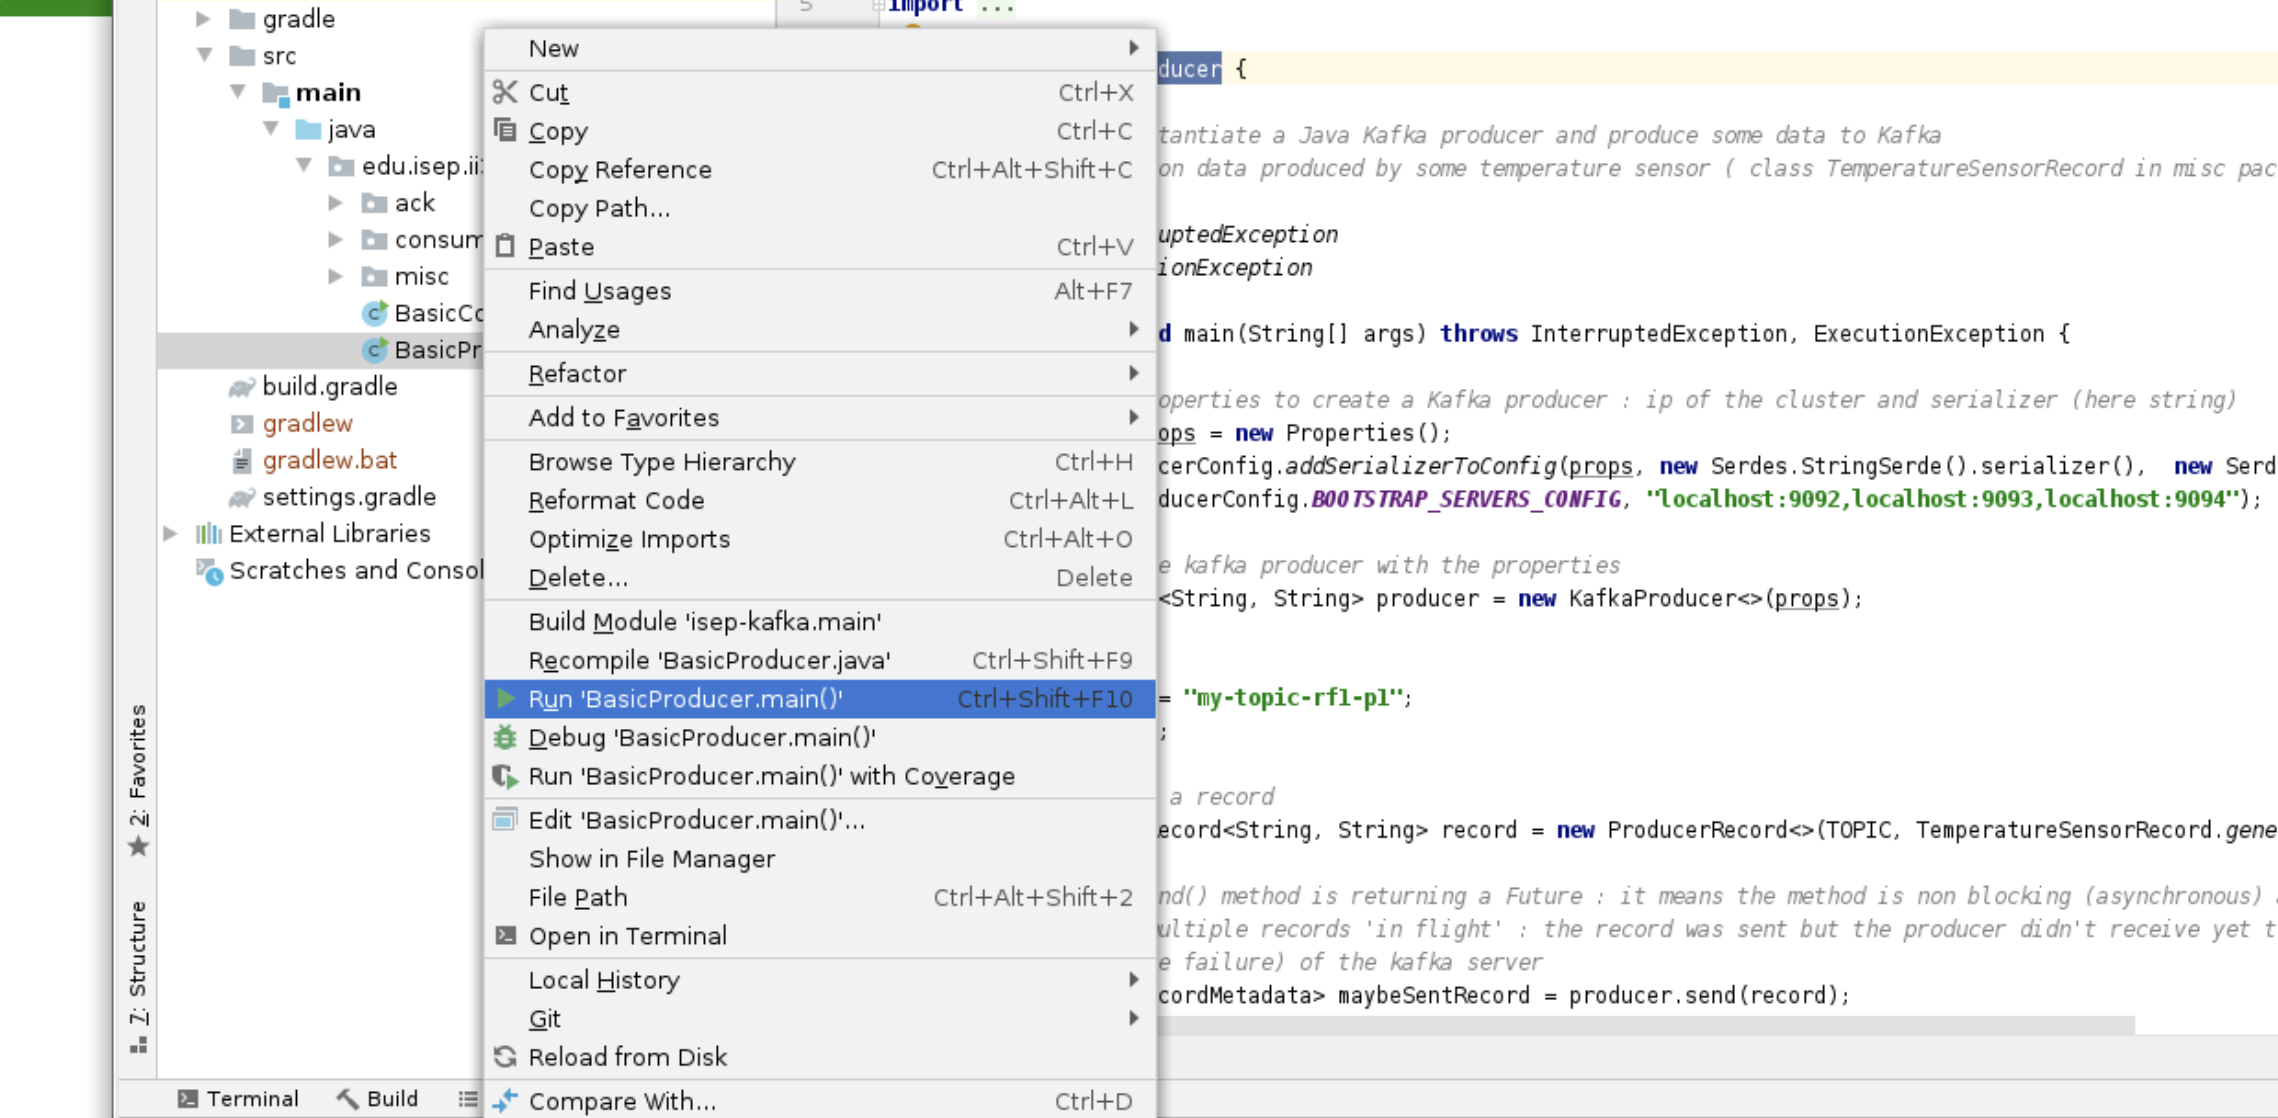
\includegraphics[width=8cm]{runJava.png}
\caption{Click right on the java class and then click on run}
\centering
\end{figure}





By checking Prometheus (localhost:9090 in chromium), type in expression field
  \begin{verbatim}
kafka_server_topic_messagesinpersec{topic='my-topic-rf1-p1'}
    \end{verbatim}

You should be able to observe the number of messages in your topic (you can click on graph to get the metric history) and get the broker\_id receiving the load (\underline{if needed scroll down the page to see the graph legend})

\begin{question}
  Based on Prometheus metric which broker id is receiving the load ? 
\end{question}

\begin{figure}[H]
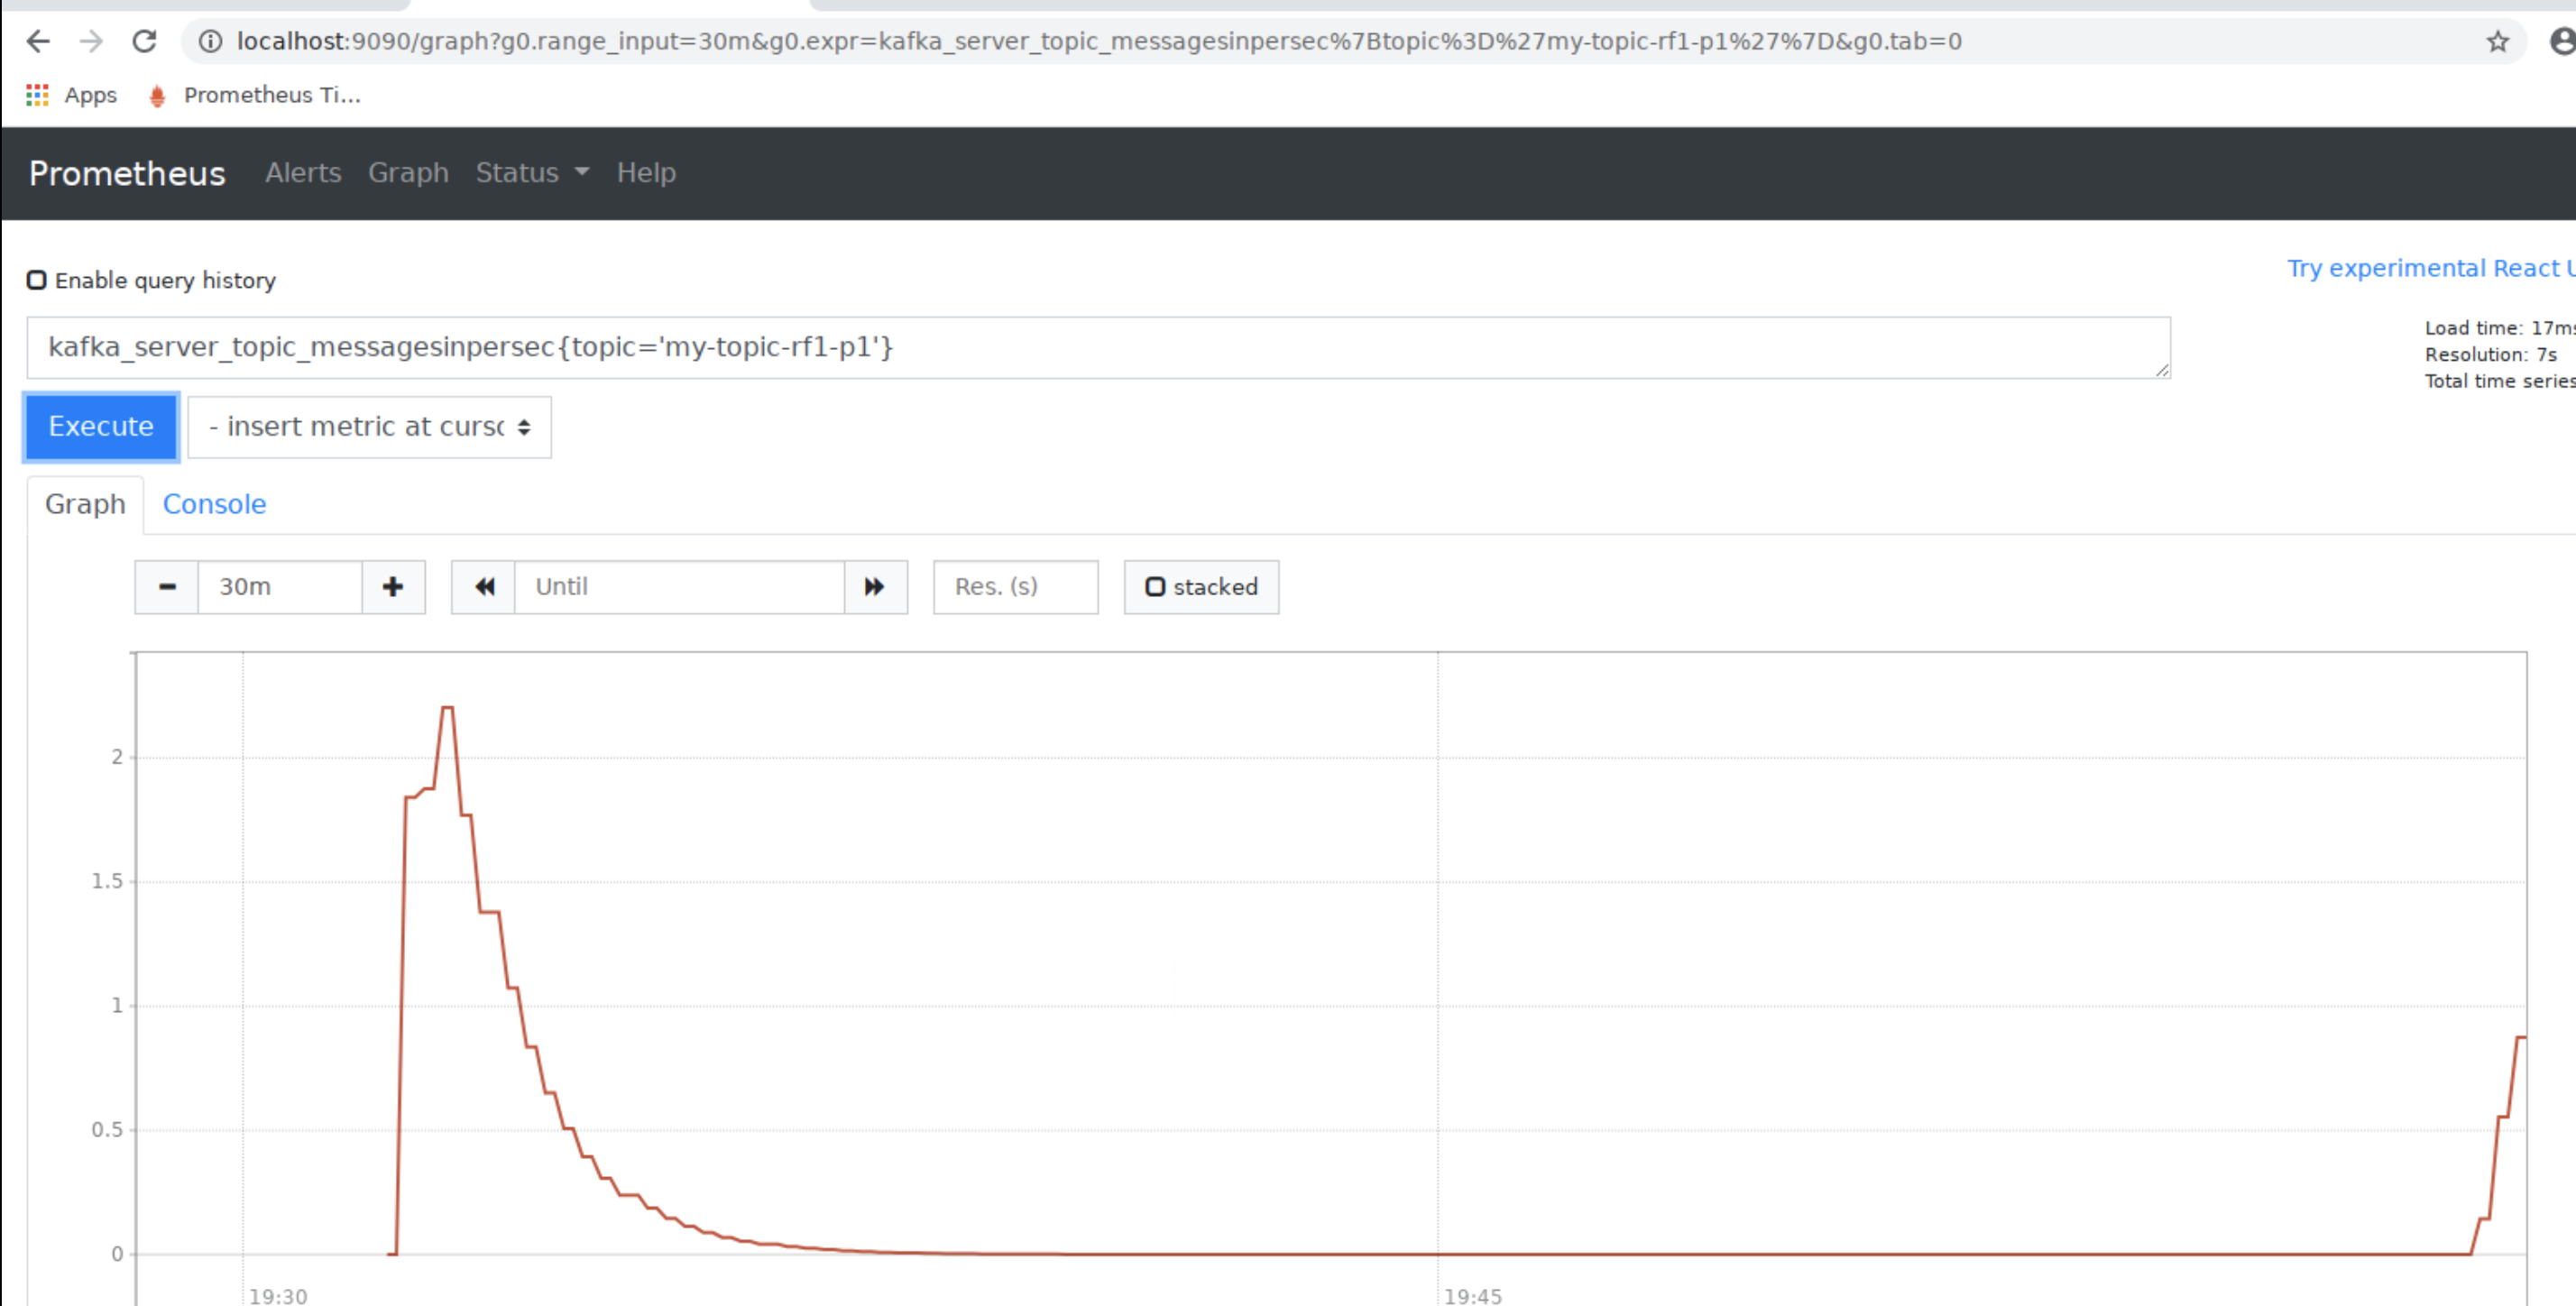
\includegraphics[width=8cm]{prometheus.png}
\caption{Number of messages per second in prometheus}
\centering
\end{figure}

\subsection{Consume messages}
With the java class edu.isep.ii3502.kafka.BasicProducer still running, run now the class


edu.isep.ii3502.kafka.BasicConsumer.
Follow the instructions in the code to consume from beginning, from tail or from a specific offset.

\begin{question}
 What's a kafka offset ?
\end{question}

\section{Experiment failure}
\subsection{Failure with non replicated topic}

Keep the producer and consumer application running. Go back to prometheus and check with the metric label which kafka broker is handling the load.

Kill the corresponding service
\begin{code}
    \begin{verbatim}
sudo systemctl stop kafka-2 # if broker_id 2 was handling the load \end{verbatim}
\end{code}


Check the messages per second in prometheus and your java application logs.

\begin{question}
 What's happening ? Is your application fault tolerant ? How to solve the issue ? 
\end{question}


Restart the killed broker 
\begin{code}
    \begin{verbatim}
sudo systemctl start kafka-2 # if broker_id 2 was handling the load \end{verbatim}
\end{code}
\subsection{Create a replicated topic}
Execute the following command to create a topic with a replicated factor of two

\begin{code}
    \begin{verbatim}
/opt/kafka/bin/kafka-topics.sh --create --topic my-topic-rf2-p1 \
--replication-factor 2 --partitions 1 --zookeeper localhost:2181 \end{verbatim}
\end{code}


Check the status of your new topic with the following command
\begin{code}
    \begin{verbatim}
/opt/kafka/bin/kafka-topics.sh --describe --topic my-topic-rf2-p1 \
--zookeeper localhost:2181 \end{verbatim}
\end{code}

Keep note of the leader id indicated.


\\
Modify the java code of the producer and consumer to change the topic name to my-topic-rf2-p1
\\


Do the same operation than the previous section and kill again the broker handling the load (change the topic name to my-topic-rf2-p1 in prometheus metric to get the broker id). What is happening, is the application now fault-tolerant ? 
\\


Recheck the status of your topic with the same command than before 
\begin{code}
    \begin{verbatim}
/opt/kafka/bin/kafka-topics.sh --describe --topic my-topic-rf2-p1 \
--zookeeper localhost:2181 \end{verbatim}
\end{code}

What's the leader id now ? 
\begin{question}
 Is the kafka replication model is a master-follower or a master-master ? 
\end{question}
\begin{question}
 Is this configuration scalable ? Why ? 
\end{question}
Stop all your running java classes.

\section{Scaling - broker side}

As you saw using prometheus, in our current configuration, one kafka broker is taking the full load when others are just standby replicas (and so we will have an issue when the load will be more important than the capacity of one server ! ). We will create a multi partitions topic to solve this issue. 
\subsection{Create the topic}

\begin{code}
\begin{verbatim}
/opt/kafka/bin/kafka-topics.sh --create --topic my-topic-rf2-p4 \
--replication-factor 2 --partitions 4 --zookeeper localhost:2181 \end{verbatim}
\end{code}

You can describe the topic 

\begin{code}
    \begin{verbatim}
/opt/kafka/bin/kafka-topics.sh --describe --topic my-topic-rf2-p4 \
--zookeeper localhost:2181 \end{verbatim}
\end{code}

Check the partitions leaders (and replicas) are well balanced between servers.


\subsection{Produce}
Modify edu.isep.ii3502.kafka.BasicProducer, TOPIC\textunderscore NAME variable to set it to my-topic-rf2-p4 and execute it.

Check application log, especially the partition and the offset of each record sent.
You can also check the number of messages per seconds using prometheus.

\begin{question}
 How the producer is choosing partition of a record ?
\end{question}

\begin{question}
By checking prometheus, why one server is receiving more messages than others ? 
\end{question}


You can now launch multiple producers (just click on run a second time) to simulate a second server producing records. 

\subsection{Consume}
Modify edu.isep.ii3502.kafka.BasicConsumer, TOPIC\textunderscore NAME variable to set it to my-topic-rf2-p4 and execute it.

You can see your consumer receiving records of all partitions.


\\
Try to launch a second consumer, you can also see that both of your consumers are receiving the same records (and so each record is proccessed two times)


\begin{question}
Is edu.isep.ii3502.kafka.BasicConsumer a scalable and a fault tolerant application ?
\end{question}


\section{Scaling - consumer side (BONUS PART)}

In order of well balance the load between consumer application we will use the consumer group feature of Kafka.


\\
Stop all java applications except one producer to my-topic-rf2-p4.
\\

Open edu.isep.ii3502.kafka.consumergroup.ConsumerWithinAConsumerGroup.
\\


Check ConsumerConfig.GROUP\textunderscore ID\textunderscore CONFIG, compare it value with the value that was set 

in edu.isep.ii3502.kafka.BasicConsumer.
\\


ConsumerWithinAConsumerGroup class is logging the partition assigned to the consumer.
\\


Execute ConsumerWithinAConsumerGroup, observe that the application is assigned to all partitions of the topic.
\\


Execute a second instance (with the first one still running) of ConsumerWithinAConsumerGroup class. What are now the partitions assigned to each application.


\\
Start now a third and fourth instances of ConsumerWithinAConsumerGroup. Observe the partitions assigned.
\\


Come back to only one instance of ConsumerWithinAConsumerGroup.  Observe the partitions assigned.


\begin{question}
(BONUS) 
Explain why edu.isep.ii3502.kafka.consumergroup.ConsumerWithinAConsumerGroup is a scalable and fault tolerant application.
\end{question}

\begin{question}
(BONUS) 
What happen if you launch 5 instances of the ConsumerWithinAConsumerGroup? Is all instances are receiving records ? Why ?
\end{question}


Stop now the last consumer and take note of the last tuple (offset, partition) read by this consumer. 


\\
Keep one producer application and wait a little bit (30 seconds). Take note of the last tuple (offset, partition) sent by your producer.


\\ 
Start one consumer application. Take note of the first (offset, partition) read by this consumer. Assert there is no message lost in your consuming application.

\begin{question}
(BONUS) 
How do you think Kafka is storing consumer offset ? 
Is the consumer application at-least-once; at-most-once or exactly once ? 
How can you have your consumer application exactly-once ? 
\end{question}


\section{Count records per sensor id}
\subsection{Complete code}
Kill all consumers running.


We now want to count records by sensor id.

Open edu.isep.ii3502.kafka.consumergroup.ConsumerCountBySensorId. Complete code to produce an output like 
\begin{code}
    \begin{verbatim}
sensor_id : 25   record_count : 25
sensor_id : 27   record_count : 32
sensor_id : 25   record_count : 26
(...)
 \end{verbatim}
\end{code}

Run now multiple instances of your application, what's the issue ? 

\begin{question}
(BONUS) 
Explain how you can partition data to avoid having data inconsistency when you have multiple instances of your application ?
\end{question}

\subsection{Add key to records}
Modify edu.isep.ii3502.kafka.BasicProducer to use sensor id as Kafka record key. You can do the following change : 

\begin{itemize}
    \item Get the output of generateRecord() method in a variable
    \item Extract the sensor id value in a new variable
    \item In the send() method, add the key argument (new ProducerRecord(TOPIC, sensorID, TemperatureSensorRecord.generateRecord())
\end{itemize}

Restart the producer and rerun multiple instances of ConsumerCountBySensorId, do you still have data inconsistency ?

\begin{question}
(BONUS) 
Explain the relationship between kafka record key and kafka partition
\end{question}

\begin{question}
(BONUS) 
Is your application with my-topic-rf2-p4 topic, consumer group and key partitionning is scalable and fault tolerant ? Why ? 
\end{question}

\section{Data consistency inside Kafka}
\begin{question}
(BONUS) 
For a topic with mulitple partitions, and a consumer reading all partitions. Do you have a global order of records (all records are read in the same order than they was sent) ? Why ? Which order guarantee do you have ? 
\end{question}


Kafka producers allows to have different mode of acknowledgement (ack setting). 

Open edu.isep.ii3502.kafka.ack.ProducerWithAck java class. 



Kafka producer have the three following ack mode : 
\begin{itemize}
    \item ack = 0 : "send and forget mode". Kafka producer are not waiting any answer from kafka server or is not doing any retry.
    \item ack = 1 : "just wait leader answer" : Kafka producer is waiting answer from the kafka leader handling the partition the record was sent. Some retries can be set in case of failure.
    \item ack = all : "wait leader and replica answers" : Kafka producer is waiting answer from the kafka leaderand replica handling the partition the record was sent. Some retries can be set in case of failure.
\end{itemize}

\begin{question}
(BONUS) 
For all ack settings (0, 1, all) indicate if it's al-least-once (so can generate duplicates); at-most-once (so can generate message lost) or exactly-once ?
\end{question}


\end{document}
